\documentclass[conference]{IEEEtran}
\IEEEoverridecommandlockouts

\usepackage{cite}
\usepackage{amsmath,amssymb,amsfonts}
\usepackage{graphicx}
\usepackage{textcomp}
\usepackage{xcolor}
\usepackage{colortbl}
\usepackage{booktabs}
\usepackage{tikz}
\usepackage{pgfplots}
\pgfplotsset{compat=1.18}
\usetikzlibrary{arrows.meta,positioning,shapes.geometric,fit}
\definecolor{ctitle}{HTML}{2c2739}
\definecolor{mypurple}{HTML}{d2cce1}
\def\BibTeX{{\rm B\kern-.05em{\sc i\kern-.025em b}\kern-.08em
    T\kern-.1667em\lower.7ex\hbox{E}\kern-.125emX}}

\begin{document}

\title{LVForge: PE Malware Detection from Strong Baselines to Deep Metric Learning\\
{\color{ctitle}A Practical and Reproducible Study}}

\author{\IEEEauthorblockN{Ly Ngoc Vu}
\IEEEauthorblockA{\textit{Industrial University of Ho Chi Minh City} \\
Ho Chi Minh City, Vietnam \\
dezzhuge@gmail.com}}

\maketitle

\begin{abstract}
This paper explains, in a practical step-by-step manner, what was built in LVForge for Windows PE malware detection and why each component was added. The previous stage of this project compared classical machine learning and text-based deep learning baselines on a large PE dataset. In this stage, the pipeline is extended with deep metric learning on top of a shared Transformer backbone (LVModel). Five variants are evaluated under the same data and training protocol: baseline, ArcFace, Contrastive, Triplet, and Multi-Similarity. Results are reported with multi-seed statistics and deployment-oriented metrics, including TPR at low FPR. The key outcome is that Multi-Similarity provides the most reliable operating profile, while ArcFace is unstable at strict low-FPR thresholds. The paper focuses on clarity and reproducibility so that first-time readers can directly understand what was done, how it was implemented, and what should be used in practice.
\end{abstract}

\begin{IEEEkeywords}
malware detection, PE files, Transformer, deep metric learning, low-FPR evaluation, reproducibility
\end{IEEEkeywords}

\section{\textcolor{ctitle}{Introduction}}
Windows PE malware detection is important in real systems where even a small false-positive rate can create major operational cost. A model with high overall accuracy may still fail under strict deployment thresholds. Therefore, this work focuses on both global metrics (Accuracy/F1/AUC) and operating-point metrics (TPR@FPR).

This paper is written as a clear ``what was built'' report for first-time readers. It consolidates knowledge from the previous project stage and the current implementation:
\begin{itemize}
\item \textbf{Previous stage:} strong baselines using Logistic Regression, Random Forest, SVC, XGBoost, and text-based deep models (LSTM, BiLSTM, DistilBERT) \cite{atc2024}.
\item \textbf{Current stage:} a unified Flax/JAX Transformer (LVModel) plus deep metric learning objectives.
\end{itemize}

\textbf{Main contributions of this paper:}
\begin{enumerate}
\item A clear transition from baseline classification to metric-learning variants in one reproducible pipeline.
\item A detailed architectural breakdown of LVModel from tensor flow to training heads.
\item A practical interpretation of results under low-FPR deployment constraints.
\end{enumerate}

\section{\textcolor{ctitle}{What Was Done: Old vs New}}
\subsection{Previous Project Stage}
The previous paper established a strong foundation on PE malware detection using:
\begin{itemize}
\item classical ML baselines (Logistic Regression, Random Forest, SVC, XGBoost),
\item ensemble methods,
\item text-based deep models (LSTM, BiLSTM, DistilBERT),
\item and a large PE dataset setting (\textasciitilde34k samples) \cite{atc2024,sorel,bodmas}.
\end{itemize}

\subsection{Current Project Stage}
In this stage, the core addition is deep metric learning on top of the same backbone and data pipeline. Instead of changing everything at once, only the objective/head is changed while keeping the encoder trunk shared. This makes comparisons fair and easier to interpret.

\section{\textcolor{ctitle}{Methodology}}
\subsection{Task and Data Setting}
The binary task is benign vs malware classification from PE-derived text-like features. The current training setting uses an imbalanced ratio near 1:19 (benign:malware), which is exactly why threshold-sensitive evaluation is required.

\subsection{LVModel Architecture (Core Encoder)}
LVModel is a Transformer encoder classifier implemented in Flax/JAX.

Let input token IDs be $\mathbf{X}\in\mathbb{N}^{B\times T}$.

\textbf{(1) Input representation}
\begin{equation}
\mathbf{H}_0 = E_{tok}(\mathbf{X}) + E_{pos}(1{:}T).
\end{equation}
This combines token embedding and positional embedding.

\textbf{(2) Multi-Head Self-Attention block}
A single dense layer computes concatenated QKV:
\begin{equation}
\mathrm{QKV}=W_{qkv}\mathbf{H}\in\mathbb{R}^{B\times T\times 3d}.
\end{equation}
Then Q, K, V are reshaped per head and attention is computed by:
\begin{equation}
\mathbf{A}=\mathrm{softmax}\left(\frac{QK^\top}{\sqrt{d_h}}\right).
\end{equation}
The attended output is projected back to model dimension $d$.

\textbf{(3) Transformer layer design (pre-norm + residual)}
Each layer uses pre-normalization and two residual paths:
\begin{align}
\tilde{\mathbf{H}} &= \mathrm{LN}(\mathbf{H}_{l-1}), \\
\mathbf{H}' &= \mathbf{H}_{l-1} + \mathrm{MHA}(\tilde{\mathbf{H}}), \\
\mathbf{H}_{l} &= \mathbf{H}' + \mathrm{FFN}(\mathrm{LN}(\mathbf{H}')).
\end{align}
The FFN is two linear layers with GELU and dropout.

\textbf{(4) Classification path}
After stacking encoder layers, sequence features are mean-pooled:
\begin{equation}
\mathbf{z}=\frac{1}{T}\sum_{t=1}^{T}\mathbf{H}_{L,t}.
\end{equation}
Then LVModel applies dense+tanh pooler, dropout, LayerNorm, and final classifier logits.

\textbf{Configuration used in experiments:}
$d_{model}=256$, heads $=8$, $d_{ff}=512$, layers $=2$, max length $=380$.

\subsection{Metric-Learning Extensions}
All variants share the same encoder trunk. For metric-learning variants, an additional projection to $d_{emb}=256$ is used, followed by LayerNorm and $\ell_2$ normalization of embeddings. Variant-specific heads/objectives are:
\begin{itemize}
\item \textbf{ArcFace:} angular margin classification \cite{arcface},
\item \textbf{Contrastive:} pair similarity/distance regularization \cite{contrastive},
\item \textbf{Triplet:} relative-distance margin optimization \cite{triplet},
\item \textbf{Multi-Similarity:} weighted hard pair optimization \cite{msloss}.
\end{itemize}

\subsection{End-to-End Pipeline}
Figure~\ref{fig:pipeline} summarizes the full workflow used in practice.
\begin{figure*}[!t]
\centering
\resizebox{\textwidth}{!}{%
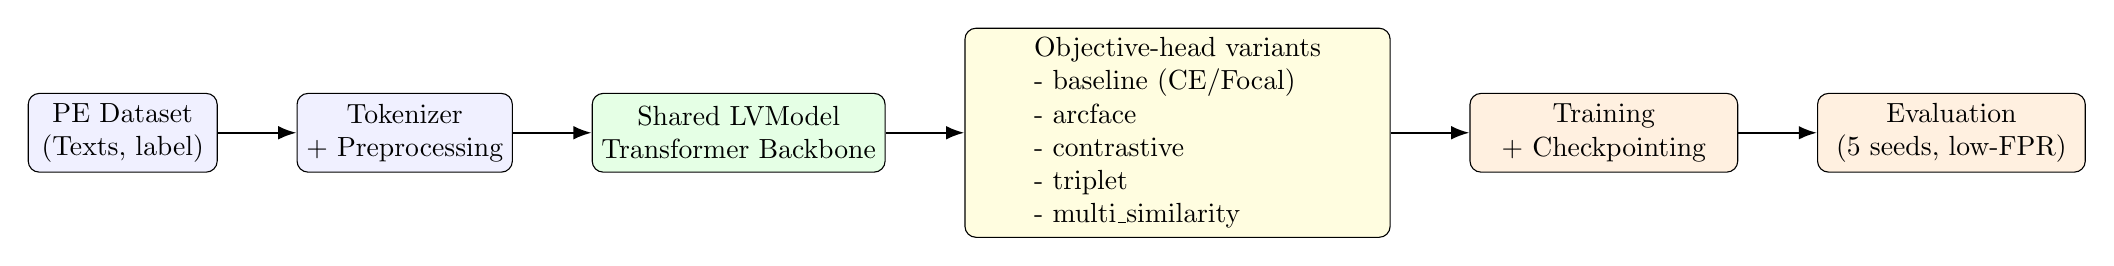
\begin{tikzpicture}[
    node distance=9mm and 10mm,
    stage/.style={draw, rounded corners, align=center, minimum height=10mm, minimum width=24mm, fill=blue!6},
    core/.style={draw, rounded corners, align=center, minimum height=10mm, minimum width=30mm, fill=green!10},
    block/.style={draw, rounded corners, align=left, minimum height=18mm, minimum width=54mm, fill=yellow!12},
    evalbox/.style={draw, rounded corners, align=center, minimum height=10mm, minimum width=34mm, fill=orange!12},
    arrow/.style={-Latex, thick}
]
    \node[stage] (data) {PE Dataset\\(Texts, label)};
    \node[stage, right=of data] (prep) {Tokenizer\\+ Preprocessing};
    \node[core, right=of prep] (backbone) {Shared LVModel\\Transformer Backbone};
    \node[block, right=of backbone] (heads) {Objective-head variants\\- baseline (CE/Focal)\\- arcface\\- contrastive\\- triplet\\- multi\_similarity};
    \node[evalbox, right=of heads] (train) {Training\\+ Checkpointing};
    \node[evalbox, right=of train] (eval) {Evaluation\\(5 seeds, low-FPR)};

    \draw[arrow] (data) -- (prep);
    \draw[arrow] (prep) -- (backbone);
    \draw[arrow] (backbone) -- (heads);
    \draw[arrow] (heads) -- (train);
    \draw[arrow] (train) -- (eval);
\end{tikzpicture}}
\caption{Unified pipeline for baseline and DML variants.}
\label{fig:pipeline}
\end{figure*}

\section{\textcolor{ctitle}{Results}}
\subsection{Reference Baselines from Previous Stage}
\begin{table}[htbp]
\caption{ML baselines from prior paper \cite{atc2024}}
\centering
\footnotesize
\begin{tabular}{lcccc}
\toprule
\rowcolor{mypurple!55}
Model & Precision & Recall & F1 & Accuracy \\
\midrule
Logistic Regression & 0.990086 & 0.990232 & 0.990111 & 0.990112 \\
Random Forest & 0.990000 & 0.990382 & 0.990402 & 0.990403 \\
SVC & 0.990000 & 0.988060 & 0.988075 & 0.988076 \\
XGBoost & 0.990000 & 0.991542 & 0.991566 & 0.991566 \\
\bottomrule
\end{tabular}
\label{tab:prior_ml}
\end{table}

\begin{table}[htbp]
\caption{Deep learning baselines from prior paper \cite{atc2024}}
\centering
\footnotesize
\begin{tabular}{lcccc}
\toprule
\rowcolor{mypurple!55}
Model & Precision & Recall & F1 & Accuracy \\
\midrule
DistilBERT & 0.9864895 & 0.9865220 & 0.9864705 & 0.986471 \\
LSTM & 0.9674135 & 0.9674490 & 0.9674130 & 0.967413 \\
BiLSTM & 0.9507005 & 0.9499545 & 0.9500705 & 0.950102 \\
\bottomrule
\end{tabular}
\label{tab:prior_dl}
\end{table}

\subsection{Current Stage: DML Comparison}
\begin{table}[htbp]
\caption{Aggregated 5-seed metrics (mean)}
\centering
\scriptsize
\setlength{\tabcolsep}{3pt}
\resizebox{\columnwidth}{!}{%
\begin{tabular}{lccccc}
\toprule
\rowcolor{mypurple!55}
Variant & Accuracy & F1 & ROC-AUC & PR-AUC & TPR@FPR=1e-2 \\
\midrule
baseline & 0.9924 & 0.9960 & 0.9983 & 0.9999 & 0.9754 \\
arcface & 0.7979 & 0.7934 & 0.9704 & 0.9984 & 0.0000 \\
contrastive & 0.9931 & 0.9964 & 0.9971 & 0.9997 & 0.9533 \\
triplet & 0.9932 & 0.9964 & 0.9969 & 0.9998 & 0.9351 \\
multi\_similarity & \textbf{0.9946} & \textbf{0.9972} & 0.9978 & 0.9999 & \textbf{0.9851} \\
\bottomrule
\end{tabular}
}
\label{tab:new_results}
\end{table}

\textbf{What these numbers mean in practice:}
\begin{itemize}
\item Multi-Similarity is the strongest overall choice for deployment.
\item Baseline is still robust and can serve as fallback/reference.
\item ArcFace is unstable for strict low-FPR operation in this setting.
\item Runtime across variants remains in a comparable practical range (about 94--133s per run variant in current setup).
\end{itemize}

\section{\textcolor{ctitle}{Discussion and Deployment Guidance}}
This work shows that adding metric learning is useful when objective choice is careful. The shared trunk + variant-head design made it easy to isolate what actually improved performance. For production-oriented usage:
\begin{enumerate}
\item prioritize operating-point metrics (TPR@FPR), not only accuracy,
\item use Multi-Similarity as primary candidate,
\item keep baseline as a stable reference,
\item recalibrate thresholds when data distribution shifts.
\end{enumerate}

\subsection{Threats to Validity}
\begin{itemize}
\item single-domain pipeline evaluation,
\item limited seed count,
\item potential calibration sensitivity under temporal drift,
\item static-feature limitations for packed/obfuscated binaries.
\end{itemize}

\section{\textcolor{ctitle}{Conclusion}}
For first-time readers, the core message is simple: this project started from strong baselines, then added a carefully controlled metric-learning extension on the same LVModel backbone. The implementation is reproducible, the architectural changes are explicit, and results indicate that Multi-Similarity gives the best operational profile under the tested PE malware setting.

\section*{Acknowledgment}
This work builds on the author's previous project stage and extends it with architecture-level and objective-level analysis.

\begin{thebibliography}{00}
\bibitem{atc2024} L. N. Vu, ``Windows Malware Detection: Exploring from Machine Learning to Text-Based Deep Learning Approaches,'' in Proc. ATC, 2024.
\bibitem{arcface} J. Deng \textit{et al.}, ``ArcFace: Additive Angular Margin Loss for Deep Face Recognition,'' CVPR, 2019.
\bibitem{msloss} X. Wang \textit{et al.}, ``Multi-Similarity Loss with General Pair Weighting for Deep Metric Learning,'' CVPR, 2019.
\bibitem{triplet} F. Schroff \textit{et al.}, ``FaceNet: A Unified Embedding for Face Recognition and Clustering,'' CVPR, 2015.
\bibitem{contrastive} R. Hadsell \textit{et al.}, ``Dimensionality Reduction by Learning an Invariant Mapping,'' CVPR, 2006.
\bibitem{sorel} A. Harang and E. M. Rudd, ``SOREL-20M: A Large Scale Benchmark Dataset for Malicious PE Detection,'' arXiv:2012.07634, 2020.
\bibitem{bodmas} BODMAS Dataset, ``Benchmark for malware analysis at scale,'' 2021.
\bibitem{calibration} C. Guo \textit{et al.}, ``On Calibration of Modern Neural Networks,'' ICML, 2017.
\bibitem{oodsecurity} S. Wang \textit{et al.}, ``A Comprehensive Survey of Out-of-Distribution Detection Methods for AI Security,'' ACM Comput. Surv., 2024.
\end{thebibliography}

\end{document}
